\subsection{Improved Open Traveling Salesman Ant Colony Optimization}
\label{subsec:aco}

The ordering layer of the framework solves the open traveling salesman problem on the cost matrix produced by the global planning layer. Given $N$ points consisting of a fixed start point $S$, $K$ intermediate goal points $\{T_1, \dots, T_K\}$, and a fixed end point $G$, the objective is to find the permutation of the $K$ goal points that minimizes the total path cost. On the basis of the ant colony optimization (ACO) metaheuristic, this paper introduces six integrated mechanisms, which are described in turn in this subsection.

\subsubsection{Virtual-Node Encoding of the Open Traveling Salesman Problem}
\label{subsec:virtual}

For the open traveling salesman problem, the start point $S$ and the end point $G$ are distinct physical locations specified by the task, and optimization is performed only on the ordering of the $K$ intermediate goal points. A naive full-permutation encoding produces invalid solutions with misaligned endpoints; if the start and end are pinned in the encoding, $S$ and $G$ are excluded from the pheromone model and local search, limiting the ability to optimize the complete solution. To this end, this paper adopts the virtual-node method to convert the open traveling salesman problem into a standard closed traveling salesman problem~\textcolor{blue}{\cite{ref32}}.

A virtual node $V = N + 1$ is introduced, and an extended cost matrix $\mathbf{D}_{\mathrm{ext}}$ of size $(N+1) \times (N+1)$ is constructed:
\begin{equation}
\mathbf{D}_{\mathrm{ext}}(i, j) =
\begin{cases}
0, & \{i, j\} = \{V, 1\} \\
0, & \{i, j\} = \{V, N\} \\
\mathrm{BIG}, & \begin{aligned}[t]
& (i = V \lor j = V) \land \\
& \{i, j\} \cap \{1, N\} = \varnothing
\end{aligned} \\
\mathbf{D}(i, j), & \text{otherwise}
\end{cases}
\label{eq:dext}
\end{equation}
where $\mathrm{BIG} = 2(N+1) \cdot \max_{i,j} \mathbf{D}(i,j)$ is a penalty strictly larger than the cost of any feasible tour, ensuring that the virtual node is not directly connected to any intermediate goal point in any near-optimal tour and is therefore forced to be adjacent only to the start and the end.

The solver runs on $\mathbf{D}_{\mathrm{ext}}$ as a standard closed traveling salesman problem, and the pheromone matrix $\bm{\tau}$ covers the full $(N+1)\times(N+1)$ space. After the solver converges, $V$ is removed from the best tour, the remaining nodes are read in tour order and reordered so that the start comes first and the end last, yielding the open visiting sequence. Relative to the boundary-fixed encoding, this transformation lets the start and end fully participate in pheromone updates and local search, allows closed-tour operators to be applied uniformly, and makes the cost evaluation simply the tour sum on $\mathbf{D}_{\mathrm{ext}}$. The heuristic visibility matrix $\bm{\eta}$ is defined as
\begin{equation}
\eta_{ij} =
\begin{cases}
\mathrm{BIG}, & \{i, j\} = \{V, 1\} \text{ or } \{V, N\} \\
\dfrac{1}{\mathbf{D}_{\mathrm{ext}}(i,j)}, & \mathbf{D}_{\mathrm{ext}}(i,j) > 0 \\
0, & \text{otherwise}
\end{cases}
\label{eq:eta}
\end{equation}
i.e., the zero-cost edges incident to $V$ are assigned a large heuristic value that strongly attracts $V$ to its required neighbors, while other pairs take the reciprocal of the extended cost. The cost of a closed tour $\bm{\sigma} = (\sigma_1, \dots, \sigma_{N+1})$ is the sum of its edge costs, including the closing edge $\sigma_{N+1} \to \sigma_1$.

\subsubsection{Max--Min Ant System Pheromone Update with Dynamic Bounds}

The Max--Min Ant System (MMAS)~\textcolor{blue}{\cite{ref23}} restricts pheromone values to an explicit interval $[\tau_{\min}, \tau_{\max}]$ to prevent unilateral domination and extinction, and concentrates deposition on elite solutions. This paper adopts this mechanism and specifies a bound-initialization and update procedure matched to the cost scale.

In each iteration, all pheromone values are first evaporated as $\tau_{ij} \leftarrow (1 - \rho) \cdot \tau_{ij}$ ($\rho$ is the evaporation rate), and pheromone is then deposited on the iteration-best tour $\bm{\sigma}_{\mathrm{iter-best}}$ and the global-best tour $\bm{\sigma}_{\mathrm{global-best}}$, respectively, as
\begin{equation}
\tau_{ij} \leftarrow \tau_{ij} + \frac{Q}{C_{\mathrm{iter}}}, \qquad
\tau_{ij} \leftarrow \tau_{ij} + \frac{Q}{C_{\mathrm{global}}}
\label{eq:deposit}
\end{equation}
where $Q$ is the deposit constant and $C$ is the corresponding tour cost. The deposit amount is inversely proportional to the tour cost and is applied symmetrically to $(i,j)$ and $(j,i)$. After deposition, the pheromone is clamped to the current interval, whose bounds are given dynamically by the global-best cost:
\begin{equation}
\tau_{\max} = \frac{1}{\rho \cdot C_{\mathrm{global}}}, \qquad
\tau_{\min} = \frac{\tau_{\max}}{N+1}
\label{eq:taumax}
\end{equation}
The initial pheromone is set to a uniform value $\tau_0$, corresponding to bounds $\tau_{\max}^{0} = 1/(\rho \cdot \tau_0 \cdot (N+1))$ and $\tau_{\min}^{0} = \tau_{\max}^{0}/(5(N+1))$, so that $\tau_0$ is not clipped during the early stage; a hard lower limit is additionally imposed on $\tau_{\min}$ to prevent low-frequency edges from underflowing to extinction under small-scale costs. Within a single iteration the update order is: evaporate, deposit according to Eq.~\textcolor{blue}{\eqref{eq:deposit}}, clamp, and recompute the bounds according to Eq.~\textcolor{blue}{\eqref{eq:taumax}}.

Dynamic bound updates are critical: as the search discovers better tours, the decrease in $C_{\mathrm{global}}$ increases $\tau_{\max}$, allowing the algorithm to express stronger confidence in its current best tour; the ratio $\tau_{\min}/\tau_{\max} = 1/(N+1)$ maintains a constant relative gap, preserving a baseline exploration probability for every edge.

\subsubsection{Ant Colony System Style Pseudo-Random Transition Rule}

The pseudo-random proportional rule of the Ant Colony System (ACS)~\textcolor{blue}{\cite{ref22}} greedily selects the best candidate with a controllable probability and explores by roulette selection otherwise, balancing convergence and diversity. This paper adopts this rule as the transition mechanism during the path-construction phase.

Concretely, when an ant at the current node $u$ selects the next node from the unvisited candidate set $\mathcal{U}$, it first computes the score of each candidate as $\mathrm{score}(v) = (\tau_{uv})^{\alpha} \cdot (\eta_{uv})^{\beta}$, where $\alpha$ and $\beta$ are the pheromone and heuristic weight exponents, respectively. It then exploits with probability $q_0$, deterministically selecting the highest-scoring candidate $v_{\mathrm{next}} = \arg\max_{v \in \mathcal{U}} \mathrm{score}(v)$, and explores with probability $1 - q_0$ by roulette selection, in which each candidate $v$ is chosen with probability $\mathrm{score}(v) / \sum_{u \in \mathcal{U}} \mathrm{score}(u)$. If all scores are zero, i.e., all remaining nodes are unreachable, an unvisited candidate is selected at random as a fallback.

As can be seen, a larger $q_0$ causes more construction steps to adopt greedy selection and thus accelerates convergence, whereas a smaller $q_0$ increases the proportion of random exploration. Pairwise distances in the obstacle-constrained cost matrix usually exhibit spatial locality, so the heuristic $\bm{\eta}$ provides reasonably reliable guidance; a moderate-to-high greedy probability therefore remains beneficial for convergence while preserving diversity.

\subsubsection{Variable Neighborhood Descent Local Search Accelerated by a Candidate List}
\label{subsec:vnd}

Although the paths constructed by ants are guided by pheromone and heuristic information, they are not necessarily locally optimal. A natural improvement is to apply local search to the tours constructed by a subset of the ants in each generation, further refining solution quality by systematically examining neighboring permutations. Variable Neighborhood Descent (VND)~\textcolor{blue}{\cite{ref24}} is precisely such a class of methods: it invokes multiple neighborhood structures in sequence, each corresponding to a class of path transformations, and switches to the next structure when the current one can no longer improve the solution, until no neighborhood yields a better solution. Existing studies have shown that hybridizing MMAS or ACS with VND is highly effective for vehicle routing problems~\textcolor{blue}{\cite{ref25}}. However, standard VND must examine $O(K^2)$ neighborhoods for each operator, and the computational cost rises rapidly as the number of goal points grows, becoming a major bottleneck. Further observation reveals that many of these examinations are fruitless: when a pair of distant nodes participates in a 2-opt exchange, it rarely yields an improvement in tour cost.

To this end, this paper first introduces a precomputed candidate list to filter out unpromising neighborhood evaluations, an idea widely used in local search for the traveling salesman problem~\textcolor{blue}{\cite{ref26}}. Specifically, for each node its $k$ nearest neighbors are preselected according to the extended cost matrix $\mathbf{D}_{\mathrm{ext}}$ and stored in a Boolean matrix. During local search, the cost change of a move is computed only when the new edges it introduces are related to candidate neighbors; otherwise the evaluation is skipped.

On this basis, VND is performed on the closed tour of the $N+1$ nodes including the virtual node, alternating among three neighborhood operators in a fixed order:
\begin{enumerate}
\item \textbf{2-opt}: reverses a contiguous subsequence of the path, replacing the original edges $(u, u^{+})$ and $(v, v^{+})$ with $(u, v)$ and $(u^{+}, v^{+})$, thereby eliminating path crossings typical of Euclidean-like costs.
\item \textbf{Relocate}: takes a node from its current position and inserts it elsewhere in the tour, shifting the intermediate nodes accordingly, which corrects cases where a node has been placed in the wrong path segment.
\item \textbf{Swap}: exchanges two nodes while keeping all others unchanged, which is applicable when two nodes happen to be assigned to each other's better positions.
\end{enumerate}
The above operators all follow the first-improvement principle in the VND loop. In each round the 2-opt, relocate, and swap operators are each executed once in the fixed order; whenever any operator yields an improvement, a new round starts, and the local search terminates when none of the three operators improves the solution in a round. Because the problem is defined on a closed tour, when a swap involves the first and last adjacent nodes of the tour, the wrap-around connection is handled through cyclic predecessor and successor indices, and adjacent swaps that cross the closing edge evaluate the three involved edges separately, rather than reusing the adjacency test for a linear path.

In terms of complexity, without pruning each VND operator would examine $O((N+1)^2)$ candidate moves; with the candidate list, each node participates in only about $O(k)$ neighborhood checks, reducing the complexity of a single operator to $O((N+1)\cdot k)$. When $k$ is much smaller than $N+1$, this effectively reduces the computation relative to full-neighborhood enumeration.

Algorithm~\textcolor{blue}{\ref{alg:vnd}} gives the complete pseudocode of candidate-list-accelerated VND, and the full flow of the VND neighborhood search is shown in Fig.~\textcolor{blue}{\ref{fig:vnd_flow}}.

\begin{algorithm}[!t]
\caption{Candidate-list-accelerated variable neighborhood descent}
\label{alg:vnd}
\begin{spacing}{0.9}
\begin{algorithmic}[1]
\REQUIRE closed tour $\bm{\sigma} = [\sigma_1, \dots, \sigma_{N+1}]$, extended cost matrix $\mathbf{D}_{\mathrm{ext}}$, candidate boolean matrix $\mathbf{C}$
\ENSURE improved tour $\bm{\sigma}$ and its cost
\STATE $\mathrm{cost} \gets$ the cost of tour $\bm{\sigma}$ under $\mathbf{D}_{\mathrm{ext}}$;
\REPEAT
\STATE $\mathrm{improved} \gets$ false;
\STATE $[\bm{\sigma}, \mathrm{cost}, \mathrm{ok}] \gets$ apply the 2-opt operator with candidate-list pruning (first-improvement);
\STATE $\mathrm{improved} \gets \mathrm{improved}$ or ok;
\STATE $[\bm{\sigma}, \mathrm{cost}, \mathrm{ok}] \gets$ apply the relocate operator with candidate-list pruning;
\STATE $\mathrm{improved} \gets \mathrm{improved}$ or ok;
\STATE $[\bm{\sigma}, \mathrm{cost}, \mathrm{ok}] \gets$ apply the swap operator with candidate-list pruning;
\STATE $\mathrm{improved} \gets \mathrm{improved}$ or ok;
\UNTIL{$\mathrm{improved} = \mathrm{false}$}
\STATE $\mathrm{cost} \gets$ the exact cost of the final tour $\bm{\sigma}$;
\RETURN $\bm{\sigma}$, $\mathrm{cost}$;
\end{algorithmic}
\end{spacing}
\end{algorithm}

\begin{figure}[!t]
\centering
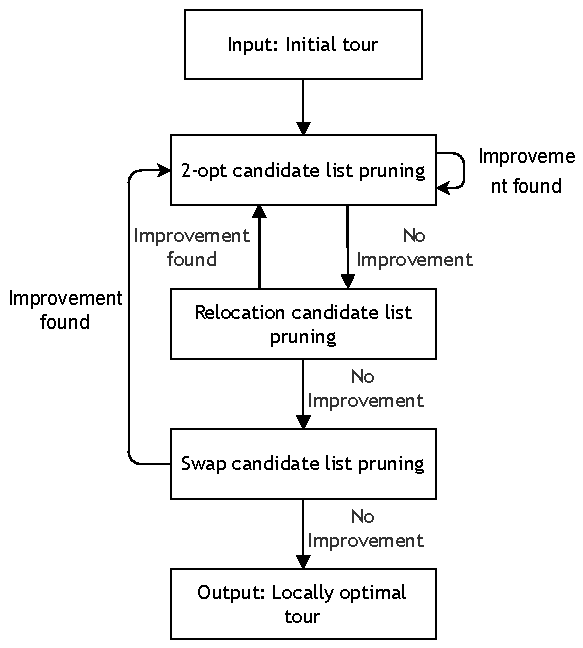
\includegraphics[width=3in]{figures/fig03_vnd_flow.pdf}
\caption{VND neighborhood search sequence flowchart.}
\label{fig:vnd_flow}
\end{figure}

\subsubsection{Sigmoid Progressive Local Search Schedule}
\label{subsec:sigmoid}

Even with candidate-list acceleration, VND local search still requires a relatively long computation time. If local search were applied to all ants in every generation, the resources of early iterations would often be wasted, since the population has not yet identified promising regions of the search space and refining low-quality tours yields limited benefit; later on, when pheromone has concentrated on high-quality regions, intensive local search becomes critical for polishing the solution. Applying local search to a fixed proportion of ants throughout the run is therefore not ideal---a low proportion slows convergence, whereas a high proportion spends computation on immature solutions. Accordingly, this paper dynamically adjusts the proportion of ants that accept VND local search along a sigmoid function:
\begin{equation}
\mathrm{optRatio}(t) = y_{\min} + (y_{\max} - y_{\min}) \cdot \frac{t^{a}}{t^{a} + (1 - t)^{a}}
\label{eq:sigmoid}
\end{equation}
where $t = (\mathrm{iter} - x_L) / (x_R - x_L)$ is the normalized position of the current iteration within the transition interval $[x_L, x_R]$; $y_{\min}$ and $y_{\max}$ are the lower and upper bounds of the local-search proportion in the early and late stages, and $a$ controls the steepness of the sigmoid curve. When $t$ precedes $x_L$, $\mathrm{optRatio}$ takes $y_{\min}$; after $x_R$ it is held at $y_{\max}$; inside the interval the proportion changes smoothly along the sigmoid curve.

This schedule smoothly shifts the search from broad exploration in the early stage to intensive refinement of high-quality solutions in the late stage, while a subset of the ants maintains construction diversity. The S-curve of $\mathrm{optRatio}(t)$ is shown in Fig.~\textcolor{blue}{\ref{fig:sigmoid}}.

\begin{figure}[!t]
\centering
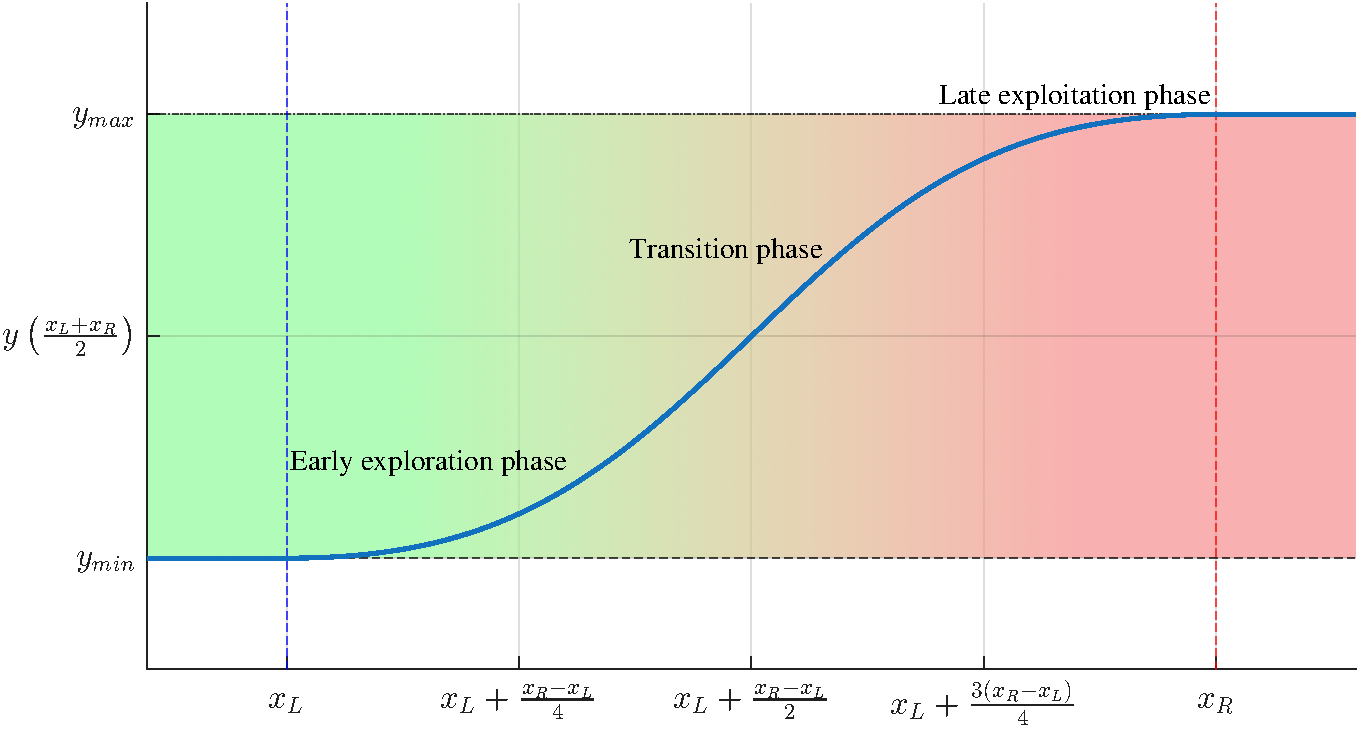
\includegraphics[width=2.5in]{figures/S_optRatio}
\caption{Sigmoid curve of $\mathrm{optRatio}(t)$ versus the iteration count.}
\label{fig:sigmoid}
\end{figure}

After the number of ants $n_{\mathrm{opt}} = \lceil n_{\mathrm{ants}} \cdot \mathrm{optRatio} \rceil$ that accept local search in the current round is determined, the specific individuals must still be selected. This paper adopts an elite--random hybrid: $n_{\mathrm{elite}} = \lceil n_{\mathrm{opt}} \cdot r_{\mathrm{elite}} \rceil$ top-ranked elite individuals are optimized first to reinforce the polishing of high-quality solutions, and the remaining $n_{\mathrm{random}} = n_{\mathrm{opt}} - n_{\mathrm{elite}}$ individuals are drawn at random from the non-elite population and optimized as well, so that promising regions outside the elite may still be discovered and a balance between exploitation and exploration is maintained. Here $r_{\mathrm{elite}}$ is the elite proportion parameter.

\subsubsection{Adaptive Stopping Criterion}

The algorithm uses the maximum iteration count $n_{\mathrm{iter}}$ as the budget ceiling so that difficult instances can still converge. On easy instances, however, convergence usually occurs far earlier, and further iterations only add computation; stopping too early, conversely, may miss better solutions. The stopping criterion must therefore distinguish ``fully converged'' from ``temporarily not improving'', and two complementary indicators are monitored simultaneously.

The first indicator is population homogeneity. When the ant colony has converged to a narrow region, the tour costs of different ants become close to each other, which can be characterized by the coefficient of variation $\mathrm{CV} = \sigma_{\mathrm{costs}} / \mu_{\mathrm{costs}}$. When $\mathrm{CV}$ falls below the preset threshold $\varepsilon_{\mathrm{CV}}$, the population is regarded as homogeneous and the chance of discovering new solutions is low.

The second indicator is stagnation of the best solution. Even if the population still has some diversity, the global best may remain near a local optimum for a long time. The algorithm therefore records the number of consecutive iterations without improvement of the global-best cost and terminates once the preset limit $\mathrm{stagn}_{\max}$ is reached.

To reduce the risk of premature stopping, the two criteria are enabled only after $\mathrm{minIter}$ iterations have been completed, because early in the search the cost variance is large and the global best is still improving rapidly, so monitoring convergence too early can misclassify normal fluctuations as convergence.

\subsubsection{Integration Summary}

In summary, the MMAS-VND-CL algorithm organizes each mechanism into a single iterative search pipeline: the extended cost matrix $\mathbf{D}_{\mathrm{ext}}$ is defined on the $N+1$ nodes including the virtual node, and both the pheromone model and the local search operate in this space. The main steps of a single iteration are as follows:
\begin{enumerate}
\item The S-curve determines the proportion of ants that accept local search in the current round;
\item All ants each construct a Hamiltonian tour covering the $N+1$ nodes according to the ACS-style pseudo-random transition rule;
\item A subset of ants is selected by the elite--random hybrid strategy, and candidate-list-accelerated VND local search is applied to their tours;
\item The current global-best tour is updated, and the adaptive stopping criterion is checked;
\item If the search continues, the pheromone is first evaporated, then deposited on the iteration-best and global-best tours, and finally clamped dynamically according to the MMAS rule.
\end{enumerate}
The search ends when the adaptive stopping condition is met. Upon termination, the virtual node $V$ is removed from the best tour, and the remaining nodes are reordered so that the start comes first and the end last, yielding the final open-path visiting sequence. The overall flow of the MMAS-VND-CL algorithm is shown in Fig.~\textcolor{blue}{\ref{fig:aco_flow}}.

\begin{figure}[!t]
\centering
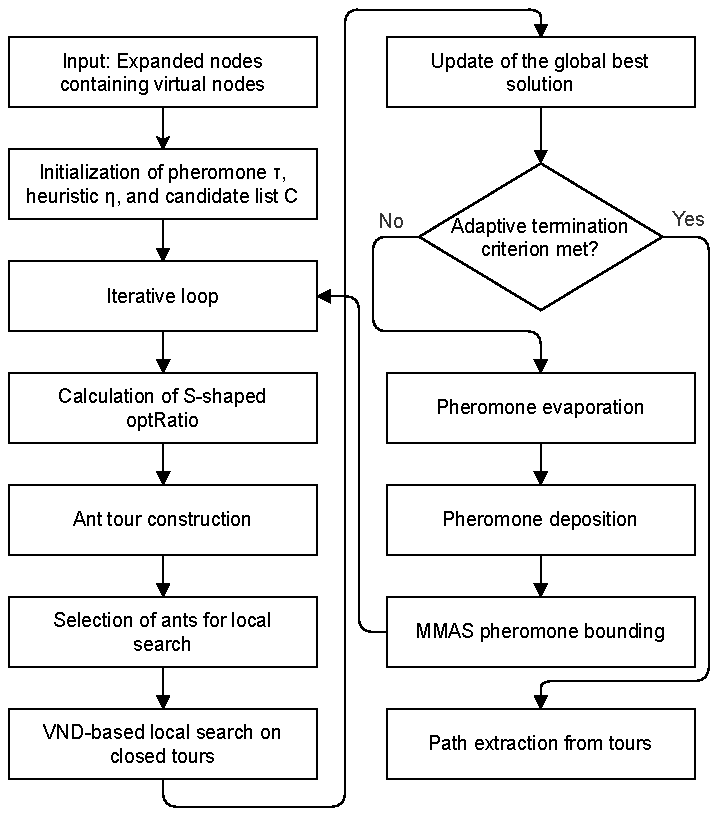
\includegraphics[width=\columnwidth]{figures/fig05_aco_flow.pdf}
\caption{Overall flowchart of the improved ant colony optimization.}
\label{fig:aco_flow}
\end{figure}

\subsection{Cooperative Optimization Framework}
\label{subsec:coop}

The preceding subsections have presented the improved A* path-finding layer and the MMAS-VND-CL ordering layer. This subsection connects the two into a complete pipeline: first construct the obstacle-constrained cost matrix, then optimize the visiting order on that matrix, and finally retrieve and concatenate the segment paths in sequence into a complete trajectory.

The geometric layer constructs the cost matrix. Given the start point, the end point, and $K$ intermediate goal points (a total of $N$ points), the shortest collision-free path is computed for every point pair; after safety simplification and arc-length-parameterized cubic spline smoothing, the Euclidean arc lengths of the continuous trajectories form the cost matrix $\mathbf{D} \in \mathbb{R}^{N \times N}$. $\mathbf{D}$ is not a Euclidean distance matrix: its elements correspond to the true obstacle-constrained traversal lengths. Pricing by smoothed arc length rather than accumulated grid steps weakens the discretization staircase effect and makes the ordering criterion closer to the actually executed travel. Construction requires $O(N^2)$ planner calls; in engineering practice a point-pair path cache can avoid repeated searches. If a point pair has no feasible path, the corresponding element is set to $\mathbf{D}(i, j) = \infty$, and if any goal is unreachable from the start, the procedure aborts and reports failure.

The ordering layer optimizes the visiting order. This layer solves the open traveling salesman problem on the numeric matrix $\mathbf{D}$ alone, without access to the map or obstacle geometry, and returns the optimal visiting sequence $\bm{\pi}^{*} = (1, \pi_2, \dots, \pi_{K+1}, N)$ together with the total cost $C(\bm{\pi}^{*})$; the segment paths of adjacent point pairs are then retrieved from the cache in this order and concatenated into a complete collision-free continuous trajectory. When $K = 0$, the problem reduces to a single-pair shortest-path query, with order $[1, N]$ and cost $\mathbf{D}(1, N)$.

Separating the two layers allows the planner and the ordering solver to be replaced independently and compared layer by layer, while the cost matrix $\mathbf{D}$ compresses the obstacle-distance topology into a compact interface, so that the ordering layer retains obstacle-avoidance feasibility without touching the grid map. The information loss is that the solver cannot tell whether two segments share the same narrow corridor, but for the objective of minimizing total cost this representation is sufficient. End to end, the system completes cost-matrix construction, open traveling salesman solving, and path retrieval in sequence; the overall architecture is shown in Fig.~\textcolor{blue}{\ref{fig:system}}.

\begin{figure}[!htbp]
\centering
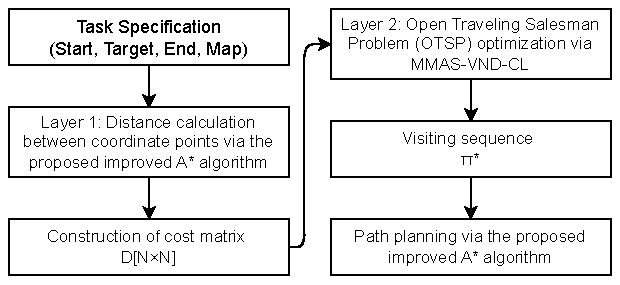
\includegraphics[width=\columnwidth]{figures/fig06_system.pdf}
\caption{Overall system architecture.}
\label{fig:system}
\end{figure}
